% Mock-up figure: two panels, for appendix/img/mock_appendix.pdf.
% Built by scripts/make_mock_figures.sh.
\documentclass[border=1pt]{standalone}
\usepackage{fourier-otf}
\usepackage{pgfplots}
\usepgfplotslibrary{groupplots}
\pgfplotsset{compat=1.18}
\definecolor{c1}{RGB}{0, 102, 173}
\definecolor{c2}{RGB}{140, 10, 28}
\begin{document}
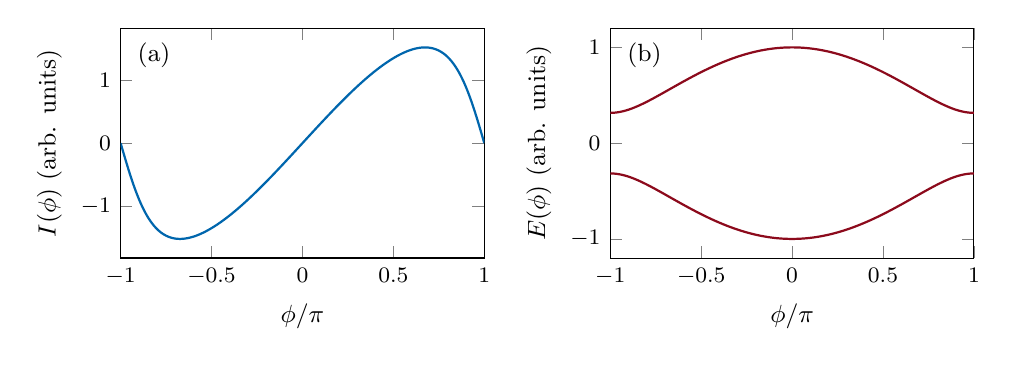
\begin{tikzpicture}
\begin{groupplot}[
    group style={group size=2 by 1, horizontal sep=16mm},
    width=62mm, height=45mm,
    xlabel={$\phi/\pi$},
    tick label style={font=\footnotesize}, label style={font=\small},
]
\nextgroupplot[ylabel={$I(\phi)$ (arb. units)}, xmin=-1, xmax=1]
\addplot[c1, thick, domain=-1:1, samples=200] {sin(deg(pi*x))/sqrt(1-0.9*sin(deg(pi*x/2))^2)};
\node[anchor=north west, font=\small] at (rel axis cs:0.02,0.98) {(a)};
\nextgroupplot[ylabel={$E(\phi)$ (arb. units)}, xmin=-1, xmax=1]
\addplot[c2, thick, domain=-1:1, samples=200] {sqrt(1-0.9*sin(deg(pi*x/2))^2)};
\addplot[c2, thick, domain=-1:1, samples=200] {-sqrt(1-0.9*sin(deg(pi*x/2))^2)};
\node[anchor=north west, font=\small] at (rel axis cs:0.02,0.98) {(b)};
\end{groupplot}
\end{tikzpicture}
\end{document}
